\graphicspath{{./results/}}
Figures \ref{fig:paperSeq},\ref{fig:rockSeq},\ref{fig:scissorsSeq} show different images sampled from each \textit{rock}, \textit{paper}, \textit{scissors} actions. Each set includes original image, background subtracted image and thresholded image after morphology on the data. The line on the subtracted image demonstrates the detected boundary for the hand.\\
It can be seen from the images that boundary is not exactly on the hand, this is the effect of Dilation using Cross kernel. For \textit{scissors} action, dilation helps connect two fingers due to shadow between them.

\begin{figure}[htp]
\begin{center}
    \subfloat[Original]{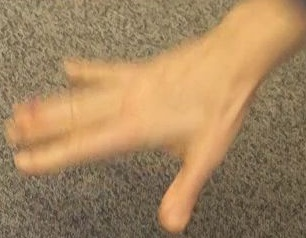
\includegraphics[width=0.25\textwidth]{13orig.jpg}}
    \subfloat[Subtracted]{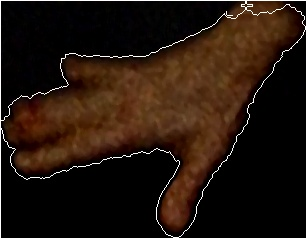
\includegraphics[width=0.25\textwidth]{13sub.jpg}}
    \subfloat[Thresholded]{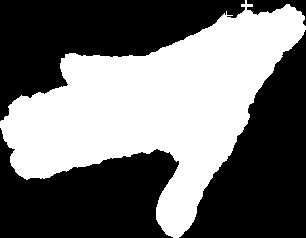
\includegraphics[width=0.25\textwidth]{13bw.jpg}}\\
    \subfloat[Original]{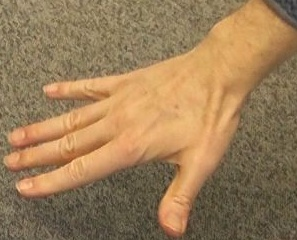
\includegraphics[width=0.25\textwidth]{18orig.jpg}}
    \subfloat[Subtracted]{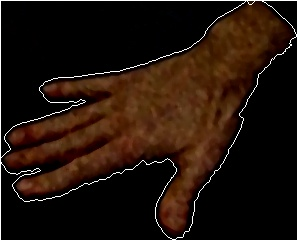
\includegraphics[width=0.25\textwidth]{18sub.jpg}}
    \subfloat[Thresholded]{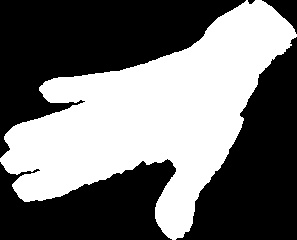
\includegraphics[width=0.25\textwidth]{18bw.jpg}}\\
    \subfloat[Original]{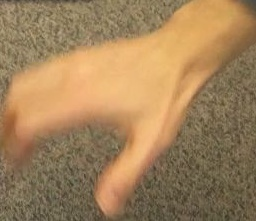
\includegraphics[width=0.25\textwidth]{115orig.jpg}}
    \subfloat[Subtracted]{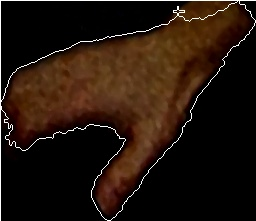
\includegraphics[width=0.25\textwidth]{115sub.jpg}}
    \subfloat[Thresholded]{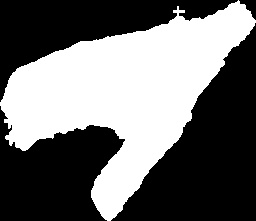
\includegraphics[width=0.25\textwidth]{115bw.jpg}}\\
    \subfloat[Motion History Image]{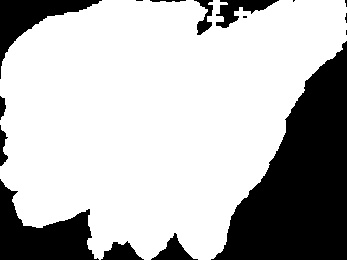
\includegraphics[width=0.25\textwidth]{1mhi.jpg}}
\end{center}
\caption{Images for paper action}
\label{fig:paperSeq}
\end{figure}

\begin{figure}[htp]
\begin{center}
    \subfloat[Original]{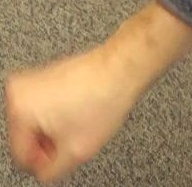
\includegraphics[width=0.25\textwidth]{43orig.jpg}}
    \subfloat[Subtracted]{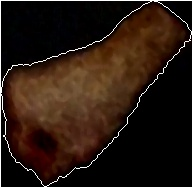
\includegraphics[width=0.25\textwidth]{43sub.jpg}}
    \subfloat[Thresholded]{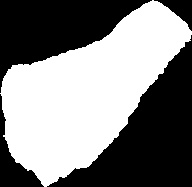
\includegraphics[width=0.25\textwidth]{43bw.jpg}}\\
    \subfloat[Original]{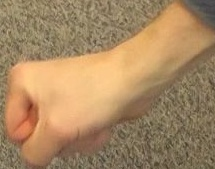
\includegraphics[width=0.25\textwidth]{64orig.jpg}}
    \subfloat[Subtracted]{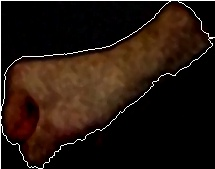
\includegraphics[width=0.25\textwidth]{64sub.jpg}}
    \subfloat[Thresholded]{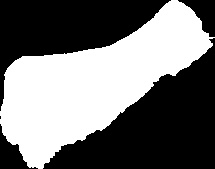
\includegraphics[width=0.25\textwidth]{64bw.jpg}}\\
    \subfloat[Original]{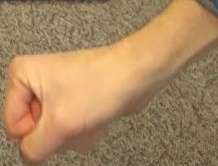
\includegraphics[width=0.25\textwidth]{69orig.jpg}}
    \subfloat[Subtracted]{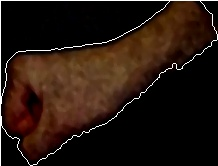
\includegraphics[width=0.25\textwidth]{69sub.jpg}}
    \subfloat[Thresholded]{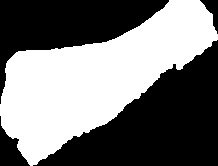
\includegraphics[width=0.25\textwidth]{69bw.jpg}}\\
    \subfloat[Motion History Image]{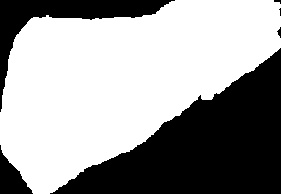
\includegraphics[width=0.25\textwidth]{6mhi.jpg}}
\end{center}
\caption{Images for rock action}
\label{fig:rockSeq}
\end{figure}

\begin{figure}[htp]
\begin{center}
    \subfloat[Original]{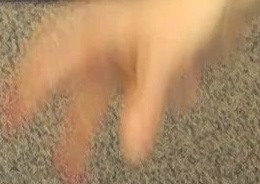
\includegraphics[width=0.25\textwidth]{82orig.jpg}}
    \subfloat[Subtracted]{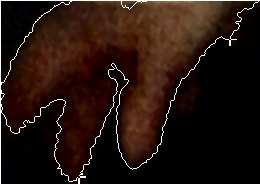
\includegraphics[width=0.25\textwidth]{82sub.jpg}}
    \subfloat[Thresholded]{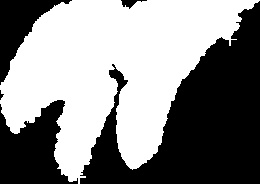
\includegraphics[width=0.25\textwidth]{82bw.jpg}}\\
    \subfloat[Original]{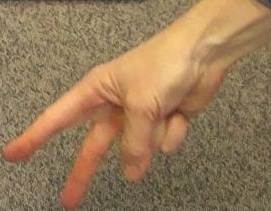
\includegraphics[width=0.25\textwidth]{89orig.jpg}}
    \subfloat[Subtracted]{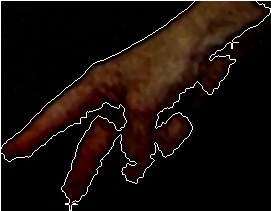
\includegraphics[width=0.25\textwidth]{89sub.jpg}}
    \subfloat[Thresholded]{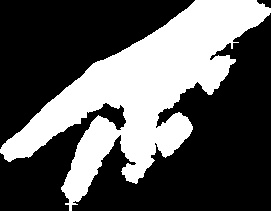
\includegraphics[width=0.25\textwidth]{89bw.jpg}}\\
    \subfloat[Original]{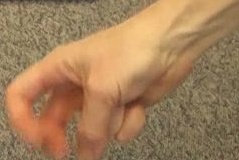
\includegraphics[width=0.25\textwidth]{817orig.jpg}}
    \subfloat[Subtracted]{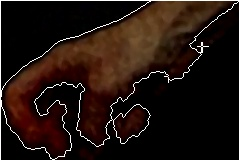
\includegraphics[width=0.25\textwidth]{817sub.jpg}}
    \subfloat[Thresholded]{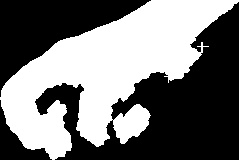
\includegraphics[width=0.25\textwidth]{817bw.jpg}}\\
    \subfloat[Motion History Image]{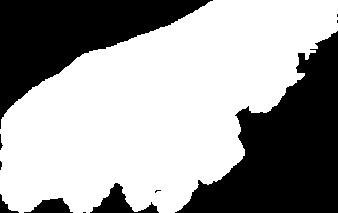
\includegraphics[width=0.25\textwidth]{8mhi.jpg}}
\end{center}
\caption{Images for scissors action}
\label{fig:scissorsSeq}
\end{figure}

\graphicspath{{./}}